\section{regs\_\-t Struct Reference}
\label{structregs__t}\index{regs\_\-t@{regs\_\-t}}
{\tt \#include $<$regs.h$>$}

Collaboration diagram for regs\_\-t:\nopagebreak
\begin{figure}[H]
\begin{center}
\leavevmode
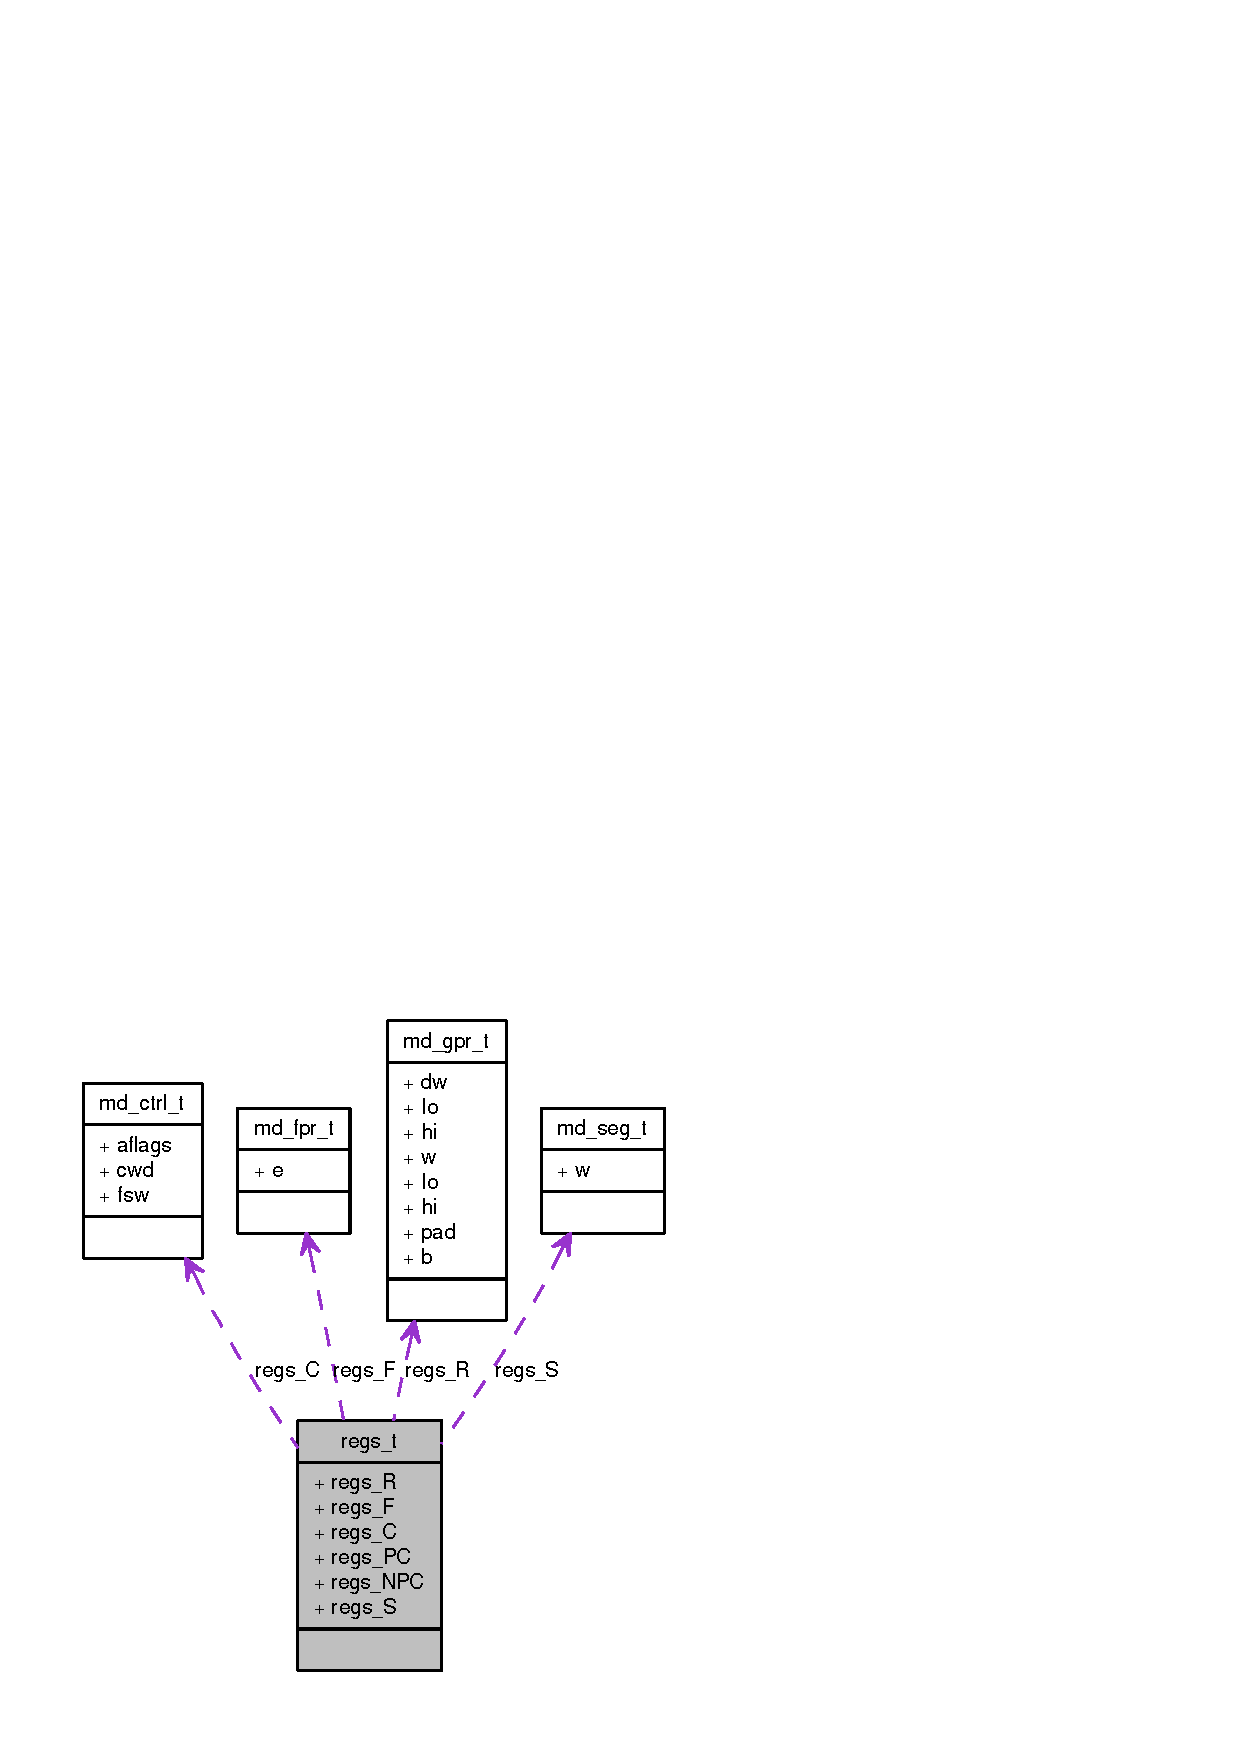
\includegraphics[width=322pt]{structregs__t__coll__graph}
\end{center}
\end{figure}
\subsection*{Public Attributes}
\begin{CompactItemize}
\item 
{\bf md\_\-gpr\_\-t} {\bf regs\_\-R}
\item 
{\bf md\_\-fpr\_\-t} {\bf regs\_\-F}
\item 
{\bf md\_\-ctrl\_\-t} {\bf regs\_\-C}
\item 
{\bf md\_\-addr\_\-t} {\bf regs\_\-PC}
\item 
{\bf md\_\-addr\_\-t} {\bf regs\_\-NPC}
\item 
{\bf md\_\-seg\_\-t} {\bf regs\_\-S}
\end{CompactItemize}


\subsection{Detailed Description}


Definition at line 99 of file regs.h.

\subsection{Member Data Documentation}
\index{regs\_\-t@{regs\_\-t}!regs\_\-C@{regs\_\-C}}
\index{regs\_\-C@{regs\_\-C}!regs_t@{regs\_\-t}}
\subsubsection[{regs\_\-C}]{\setlength{\rightskip}{0pt plus 5cm}{\bf md\_\-ctrl\_\-t} {\bf regs\_\-t::regs\_\-C}}\label{structregs__t_08bd9de629360f171b32e08c4106b46f}




Definition at line 102 of file regs.h.\index{regs\_\-t@{regs\_\-t}!regs\_\-F@{regs\_\-F}}
\index{regs\_\-F@{regs\_\-F}!regs_t@{regs\_\-t}}
\subsubsection[{regs\_\-F}]{\setlength{\rightskip}{0pt plus 5cm}{\bf md\_\-fpr\_\-t} {\bf regs\_\-t::regs\_\-F}}\label{structregs__t_199e4c2554e7b45f974cf6ecd51853ec}




Definition at line 101 of file regs.h.\index{regs\_\-t@{regs\_\-t}!regs\_\-NPC@{regs\_\-NPC}}
\index{regs\_\-NPC@{regs\_\-NPC}!regs_t@{regs\_\-t}}
\subsubsection[{regs\_\-NPC}]{\setlength{\rightskip}{0pt plus 5cm}{\bf md\_\-addr\_\-t} {\bf regs\_\-t::regs\_\-NPC}}\label{structregs__t_70500e5215c4ebb383c43c05a670346c}




Definition at line 104 of file regs.h.

Referenced by core\_\-oracle\_\-t::complete\_\-flush(), emergency\_\-recovery(), core\_\-oracle\_\-t::exec(), md\_\-fetch\_\-next\_\-pc(), core\_\-oracle\_\-t::pipe\_\-flush(), core\_\-oracle\_\-t::recover(), sim\_\-fastfwd(), sim\_\-main(), core\_\-fetch\_\-DPM\_\-t::step(), core\_\-commit\_\-STM\_\-t::step(), and core\_\-commit\_\-DPM\_\-t::step().\index{regs\_\-t@{regs\_\-t}!regs\_\-PC@{regs\_\-PC}}
\index{regs\_\-PC@{regs\_\-PC}!regs_t@{regs\_\-t}}
\subsubsection[{regs\_\-PC}]{\setlength{\rightskip}{0pt plus 5cm}{\bf md\_\-addr\_\-t} {\bf regs\_\-t::regs\_\-PC}}\label{structregs__t_c6889ccce9099e2fbf701f7fb78cedf1}




Definition at line 103 of file regs.h.

Referenced by core\_\-oracle\_\-t::complete\_\-flush(), emergency\_\-recovery(), core\_\-oracle\_\-t::exec(), md\_\-fetch\_\-next\_\-pc(), core\_\-oracle\_\-t::recover(), core\_\-oracle\_\-t::reset\_\-execution(), sim\_\-fastfwd(), sim\_\-main(), and sim\_\-post\_\-init().\index{regs\_\-t@{regs\_\-t}!regs\_\-R@{regs\_\-R}}
\index{regs\_\-R@{regs\_\-R}!regs_t@{regs\_\-t}}
\subsubsection[{regs\_\-R}]{\setlength{\rightskip}{0pt plus 5cm}{\bf md\_\-gpr\_\-t} {\bf regs\_\-t::regs\_\-R}}\label{structregs__t_09f6c8b44a3f08bc13e36c7b9a11a642}




Definition at line 100 of file regs.h.\index{regs\_\-t@{regs\_\-t}!regs\_\-S@{regs\_\-S}}
\index{regs\_\-S@{regs\_\-S}!regs_t@{regs\_\-t}}
\subsubsection[{regs\_\-S}]{\setlength{\rightskip}{0pt plus 5cm}{\bf md\_\-seg\_\-t} {\bf regs\_\-t::regs\_\-S}}\label{structregs__t_c50740591e2ad9de1d2d5b124d78f67b}




Definition at line 105 of file regs.h.

The documentation for this struct was generated from the following file:\begin{CompactItemize}
\item 
{\bf regs.h}\end{CompactItemize}
